\documentclass[../DS02.tex]{subfiles}%
\graphicspath{{./figures/}}%

\begin{document}%
\section[24]"E"{Circuit de résistances}

\enonce{%
	On considère le circuit ci-dessous~:
	\begin{figure}[htbp!]
		\centering
		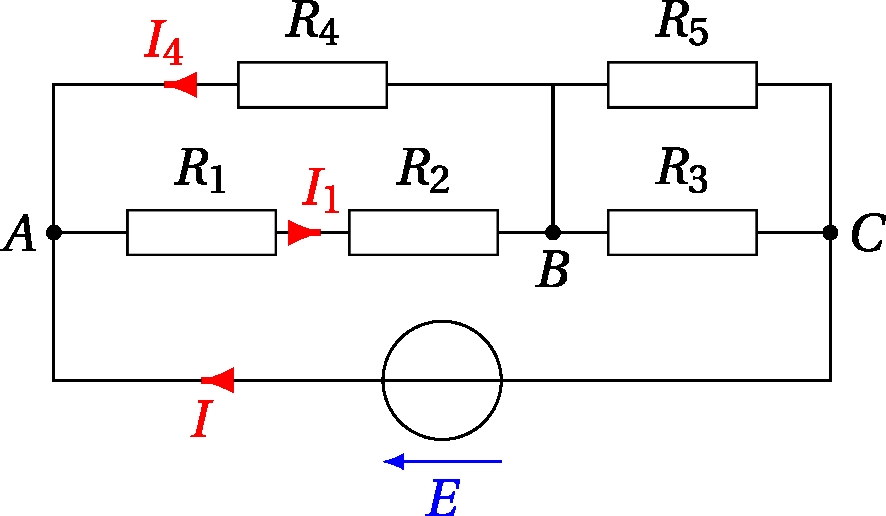
\includegraphics[width=.4\linewidth]{circ_plain}
	\end{figure}
}%

\QR[5]{%
	Comment définit-on des résistances en série ? en parallèle~? Déterminer alors,
	parmi les 5 résistances du circuit ci-dessus, lesquelles sont en série et en
	parallèle.
}{%
	Des résistances sont en série si elles \textbf{partagent une borne} \pt{1} qui
	\textbf{n'est pas un nœud} \pt{1}. Elles sont en parallèle si elles
	\textbf{partagent leurs deux bornes} \pt{1}.
	\smallbreak
	Dans ce circuit, on a $R_1$ et $R_2$ en série \pt{1}, et $R_3$ et $R_5$ en
	parallèle \pt{1}.
}%

\QR[4]{%
	En considérant que toutes les résistances ont la même valeur $R$, exprimer en
	fonction de $R$ la résistance équivalente $R_{AB}$.
}{%
	On commence par l'association série entre $R_1$ et $R_2$, qu'on appelle
	$R\ind{eq,1} = 2R$ \pt{1}. Celle-ci est en parallèle avec $R_4$. Ainsi,
	\begin{DispWithArrows*}
		\frac{1}{R_{AB}} &\stm{=} \frac{1}{R_4} + \frac{1}{R\ind{eq,1}}
		\Arrow{$R_4 = R$\\$R\ind{eq,1} = 2R$}
		\\\Lra
		\frac{1}{R_{AB}} &= \frac{2}{2R} + \frac{1}{2R} = \frac{3}{2R}
		\CArrow{$(\cdot)^{-1}$}
		\\\Lra
		\Aboxed{R_{AB} &\stm{=} \frac{2R}{3}}
	\end{DispWithArrows*}
	\pt{1} pour un schéma.
}%

\QR[4]{%
	Exprimer de même les résistances équivalentes $R_{BC}$ et $R_{AC}$ en fonction
	de $R$.
}{%
	\smallbreak
	\vspace{-25pt}
	\noindent
	\begin{minipage}[c]{.65\linewidth}
		$R_{BC}$ est l'assocation en parallèle de $R_5$ et $R_3$. D'après ce qui
		précède, on obtient alors
		\[
			R_{BC} = \frac{R^2}{2R}
			\Lra
			\boxed{R_{BC} \stm{=} \frac{R}{2}}
		\]
		Enfin, $R_{AC} = R_{AB} + R_{BC}$, soit
		\[
			\boxed{R_{AC} \stm{=} \frac{7}{6}R}
		\]
	\end{minipage}
	\hfill
	\begin{minipage}[c]{.32\linewidth}
		\begin{center}
			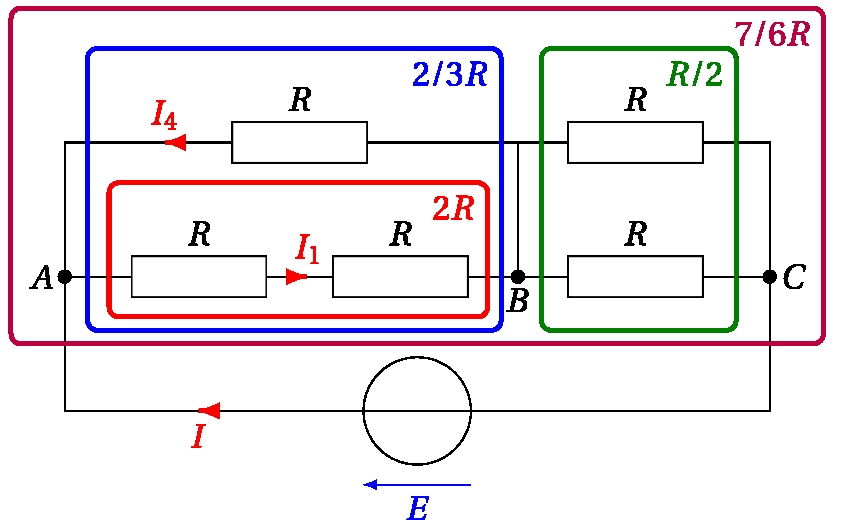
\includegraphics[width=\linewidth]{circ_req}
			\captionof{figure}{\protect\pt{1}+\protect\pt{1}}
		\end{center}
	\end{minipage}
}%

\QR[6]{%
	Exprimer les tensions $u_{AB}$ et $u_{CB}$ en fonction de $E$.
}{%
	\smallbreak
	\vspace{-25pt}
	\noindent
	\begin{minipage}[c]{.70\linewidth}
		Avec un schéma équivalent, on observe que $u_{AB}$ s'obtient par pont diviseur
		de tension, tel que~:
		\begin{gather*}
			u_{AB} \stm{=} \frac{R_{AB}}{R_{AB} + R_{BC}}E \stm{=} \frac{4}{7}E
		\end{gather*}
	\end{minipage}
	\hfill
	\begin{minipage}[c]{.24\linewidth}
		\begin{center}
			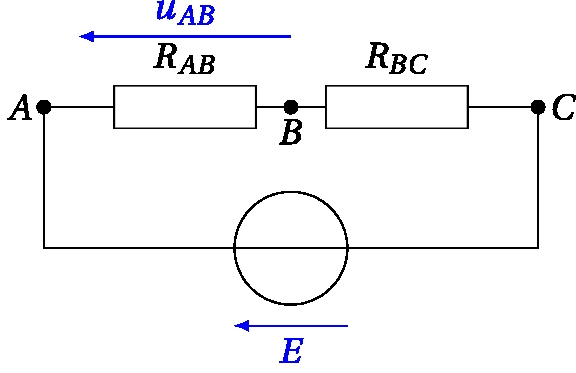
\includegraphics[width=\linewidth]{circ_uab}
			\captionof{figure}{\protect\pt{1}}
		\end{center}
	\end{minipage}
	\smallbreak
	\noindent
	\begin{minipage}[c]{.70\linewidth}
		Pour $u_{CB}$, en faisant attention au sens de la flèche, on obtient
		\begin{gather*}
			u_{CB} \stm{=} - \frac{R_{BC}}{R_{AB} + R_{BC}}E \stm{=} -\frac{3}{7}E
		\end{gather*}
	\end{minipage}
	\hfill
	\begin{minipage}[c]{.24\linewidth}
		\begin{center}
			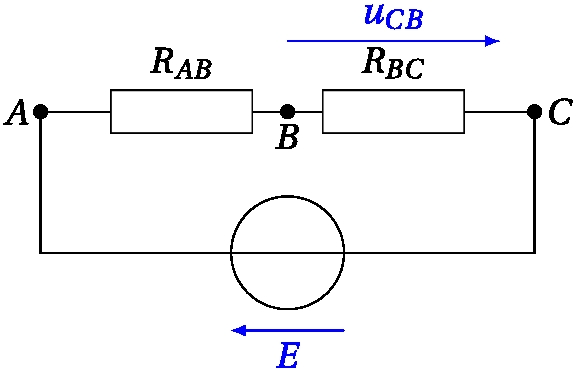
\includegraphics[width=\linewidth]{circ_ucb}
			\captionof{figure}{\protect\pt{1}}
		\end{center}
	\end{minipage}
	% \noindent
	% \begin{minipage}[c]{.48\linewidth}
	% 	\begin{center}
	% 		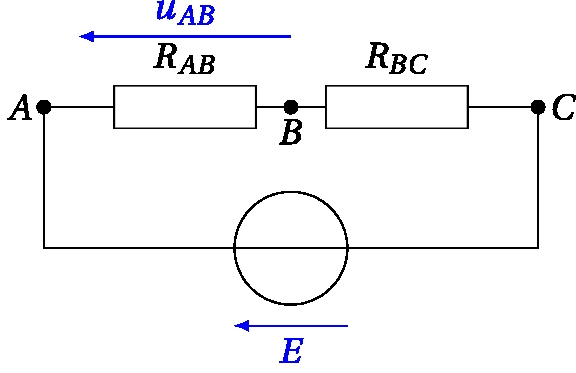
\includegraphics[width=.5\linewidth]{circ_uab}
	% 		\captionof{figure}{\protect\pt{1}}
	% 	\end{center}
	% \end{minipage}
	% \hfill
}%

\QR[5]{%
	Exprimer les intensités $I_1$ et $I_4$ en fonction de $I$.
}{%
	\smallbreak
	\vspace{-25pt}
	\noindent
	\begin{minipage}[c]{.65\linewidth}
		Avec un pont diviseur de courant, on obtient aisément~:
		\[
			I_1 \stm{=} \frac{R_{AB}}{2R}I \stm{=} \frac{1}{3}I
		\]
		De même, en faisant attention au signe~:
		\[
			I_4 \stm{=} -\frac{R_{AB}}{R}I \stm{=} -\frac{2}{3}I
		\]
	\end{minipage}
	\hfill
	\begin{minipage}[c]{.32\linewidth}
		\begin{center}
			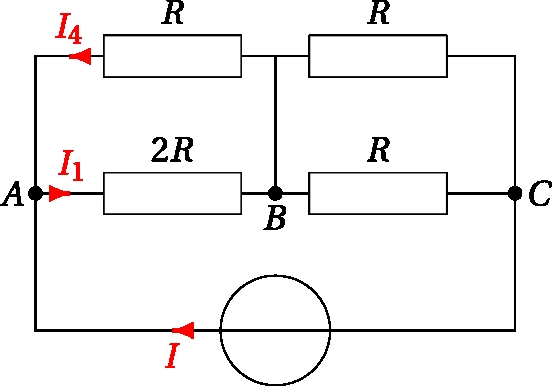
\includegraphics[width=\linewidth]{circ_divcour}
			\captionof{figure}{\protect\pt{1}}
		\end{center}
	\end{minipage}
}%

\end{document}
